% !TEX program = pdflatex
\documentclass[journal,twoside,web]{ieeecolor}
\usepackage{generic}
\usepackage{cite}
\usepackage{amsmath,amssymb,amsfonts}
\usepackage{algorithmic}
\usepackage{graphicx}
\usepackage{textcomp}
% Chinese draft support (minimal; keep IEEEtran layout unchanged).
% IMPORTANT: compile with pdfLaTeX (not XeLaTeX/LuaLaTeX) to avoid font/metric changes.
\usepackage{iftex}
\ifPDFTeX
  \usepackage{CJKutf8}
  \AtBeginDocument{\begin{CJK*}{UTF8}{gbsn}}
  \AtEndDocument{\end{CJK*}}
\else
  % Fallback for editors configured to use XeLaTeX: enable CJK rendering to avoid
  % "Unicode character not set up" errors. Output metrics may differ from pdfLaTeX.
  \usepackage{xeCJK}
  \IfFontExistsTF{Songti SC}{%
    \setCJKmainfont{Songti SC}
  }{%
    \IfFontExistsTF{SimSun}{%
      \setCJKmainfont{SimSun}
    }{%
      \setCJKmainfont{STSong}
    }%
  }%
  \PackageWarningNoLine{tii-articles-template}{For closest IEEE style, compile with pdfLaTeX instead of XeLaTeX/LuaLaTeX}
\fi
\def\BibTeX{{\rm B\kern-.05em{\sc i\kern-.025em b}\kern-.08em
    T\kern-.1667em\lower.7ex\hbox{E}\kern-.125emX}}
\markboth{\journalname, VOL. XX, NO. XX, XXXX}
{Author \MakeLowercase{\textit{et al.}}: Title}
\begin{document}
\title{面向自动化数控编程的知识图谱增强大语言模型代码生成方法}
\author{First A. Author, \IEEEmembership{Fellow, IEEE}, Second B. Author, and Third C. Author, Jr., \IEEEmembership{Member, IEEE}
\thanks{This paragraph of the first footnote will contain the date on 
which you submitted your paper for review. It will also contain support 
information, including sponsor and financial support acknowledgment. For 
example, ``This work was supported in part by the U.S. Department of 
Commerce under Grant BS123456.'' }
\thanks{The next few paragraphs should contain 
the authors' current affiliations, including current address and e-mail. For 
example, F. A. Author is with the National Institute of Standards and 
Technology, Boulder, CO 80305 USA (e-mail: author@boulder.nist.gov). }
\thanks{S. B. Author, Jr., was with Rice University, Houston, TX 77005 USA. He is 
now with the Department of Physics, Colorado State University, Fort Collins, 
CO 80523 USA (e-mail: author@lamar.colostate.edu).}
\thanks{T. C. Author is with 
the Electrical Engineering Department, University of Colorado, Boulder, CO 
80309 USA, on leave from the National Research Institute for Metals, 
Tsukuba, Japan (e-mail: author@nrim.go.jp).}}

\maketitle

\begin{abstract}
大语言模型在语义理解和推理方面表现突出，为制造业通过自然语言驱动自动化编程提供了新思路。考虑到数控编程深度依赖工艺知识与安全规则，目前的生成手段在保证代码质量和生成受控方面还存在局限。本文介绍一种面向具身智能场景的通过知识图谱增强模型能力的数控代码生成方案，利用结构化知识引导生成过程。研究者将编程流程拆解为意图解析、参数补全和程序生成三个环节。在这一过程中，利用自反思机制提升对加工需求的理解精度，并在知识图谱的辅助下完成工艺参数的逻辑推理。通过模板化构建和多层校验，能够确保生成的代码符合工业生产的安全标准。实验结果证实，这套方案有效提高了模型处理复杂任务时的可靠程度，为工业领域应用大语言模型提供了实用参考。
\end{abstract}

\begin{IEEEkeywords}
大语言模型, 知识图谱, G代码生成, 具身智能，数控系统
\end{IEEEkeywords}

\section{Introduction}
\label{sec:introduction}

离散制造正朝着柔性化与高度定制化的方向快速发展，促使数控编程从传统的人工离线编程转变为任务导向的交互式自动处理。相比于依赖固定流程和人工核验的旧有模式，这种方式需要处理由语义需求和生产要素构成的复杂环境。即使加工意图一致，也需要针对不同的设备差异和现场状态，实时调整路径方案与安全限制。在多品种生产场景下，操作员通常仅提供有关加工特征和性能偏好的概括性指令。系统则必须将这些高层意图转化为包含坐标设置、刀具补偿及运动控制在内的底层细节，并严防干涉或超程等风险。此外，代码生成并非单次完成，而是通过持续的验证与反馈实现性能提升。由于此类任务涉及精准的意图解析、参数推理以及能够自我修正的逻辑循环，其复杂程度已明显高于传统规则驱动手段的处理范围。

解决这些难题需要构建具备深度理解和知识迁移能力的智能系统。与传统手段相比，大模型（Large Language Model, LLM）在逻辑推理及知识应用上表现更为优异，能够通过交互方式明确加工意图并收集参数，进而降低编程难度。即便如此，工业控制对安全性要求极高，模型产出的结果可能存在逻辑缺失或违反控制器规范的情况，影响最终程序的稳定性。为了增强生成过程的可控程度，一种有效途径是将工艺规则和设备能力整理为结构化知识，并与生成机制相融合。在构建阶段，系统以工艺模板为核心，通过知识引导完成逻辑校验与代码输出。随后，利用多层验证策略自动识别并纠正潜在错误。通过这一套包含理解、生成与校验的完整流程，可以显著提升代码的可靠性及其在工程现场的实用性。

关于从自然语言到G代码的自动转化，现有的研究方向主要集中在两个领域。其中一类依靠预设规则与工艺模板，具备较高的稳定程度，但面对多样的表达需求时维护成本较高，难以适应复杂的加工约束。另一类则利用大型模型进行直接转化，虽然操作灵活，但在格式规范以及逻辑一致性上表现欠缺，容易产出参数超限的指令。为了改善这些状况，一些尝试侧重于通过复杂的提示策略和自反思机制引导模型优化输出。即便如此，这类手段通常需要设计冗长的提示内容，且缺乏对工艺细节与安全条件的统一表述，无法清晰展现从加工工艺到物理限制的层级关联。这也导致当结果出现偏差时，系统难以判定究竟是意图识别还是逻辑推理环节出现了偏差。以常见的车削加工为例，同一项任务受到刀具配置、加工余量、进给速度和空间运动限制等多重因素影响。任何微小的逻辑冲突都可能在后续环节中放大并引发生产风险。鉴于此，本文的研究目标是建立一套可控、可解释且安全可靠的自动化编程方案。该方案利用结构化数据定义工艺限制，结合多环节推理和分级校验，实现了从自然语言到加工代码的完整逻辑。

大模型在数控编程中的任务求解可以类比专业人员的逐步学习和调试过程。在应对复杂加工任务前，专业人员通常先建立对基础语法及加工循环的认知，随后才开始处理涉及工艺参数和作业限制的高级决策。这种由浅入深的方法能确保程序在受控状态下逐渐完善。类似的，如果要求模型直接根据模糊指令产出结果，容易在工艺逻辑上出现偏差。将任务拆解为多个可验证的中间环节，并在各阶段引入知识约束，则更有利于产出可靠的代码。例如在处理车削任务时，系统不仅要解析几何特征，还需推导出进给逻辑并执行参数校验。因此，面对复杂的制造环境，模型需要采用逐层细化的推理策略，在工程规则的引导下整合各项要素，最终产出安全的程序。这种逻辑在系统层面表现为由感知到决策再到执行的优化模式，为后续算法的协同设计提供了统一的解释框架。

基于上述分析，本文提出一种面向自动化数控编程的知识图谱增强大语言模型代码生成方法。如图\ref{fig:system-framework}所示，该方案以具身智能为系统组织视角，在结构化知识的约束下建立了多环节G代码生成流程。系统首先利用自反思机制解析工艺意图并提取关键信息，随后通过交互补全策略完善加工参数。接着在知识引导下完成模板匹配和代码渲染，确保产出的指令符合工业标准。最后利用多级验证及纠错程序对结果进行评估，从而提升程序的可靠程度。这种方式将模型的语义理解与工程受控机制有机结合，为复杂加工任务提供了可追溯且可应用的技术路径。

\begin{figure}[!t]
\centering
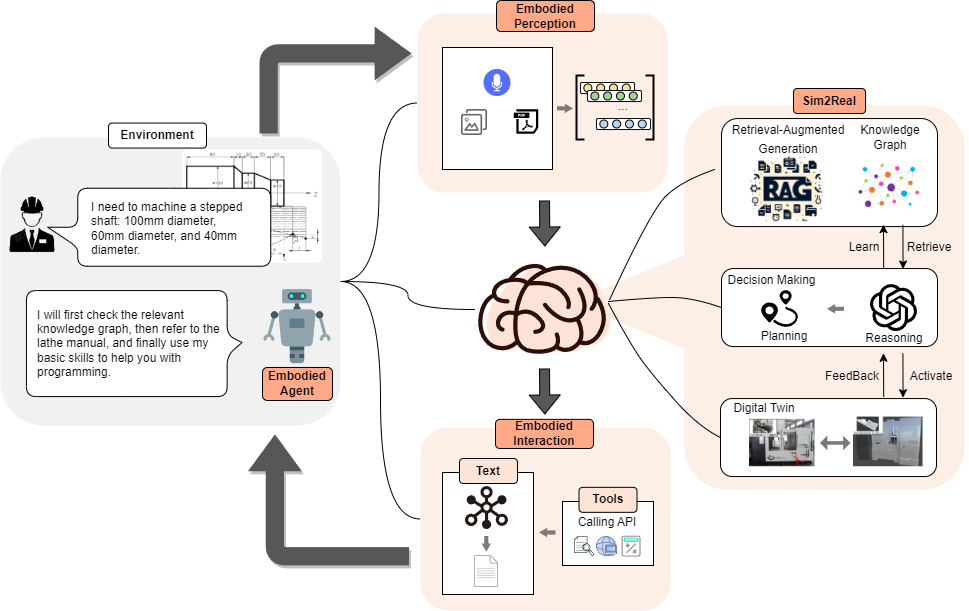
\includegraphics[width=0.98\columnwidth]{system-framework.png}
\caption{Illustration of the proposed embodied-intelligence CNC programming framework empowered by a knowledge graph and LLMs. \textbf{Environment}: user instructions and machining context. \textbf{Embodied Perception}: multimodal parsing of task inputs. \textbf{Embodied Agent}: LLM-centered planning and reasoning supported by the knowledge graph (with optional documentation search). \textbf{Embodied Interaction}: tool and API invocation with code generation outputs. \textbf{Sim2Real}: digital-twin-based verification and feedback for iterative refinement.}
\label{fig:system-framework}
\end{figure}

本文的主要贡献如下：
\begin{enumerate}
\item 提出知识图谱增强的数控代码生成框架，将生产要素进行结构化整合，并以完整的逻辑循环支撑自动化流程。
\item 设计意图识别与参数补全方案，实现对模糊指令的鲁棒理解，在降低沟通成本的同时确保参数完整。
\item 建立知识引导的模板匹配机制，在确保代码规范的前提下实现受控生成，并提供清晰的逻辑支撑。
\item 构建多级递进的验证与纠错体系，从多个维度约束输出质量，提升了加工过程的可靠程度。
\end{enumerate}

\section{Related Works}
\label{sec:related-works}

本节梳理大模型在智能制造与数控编程中的应用进展，评述受控代码生成的技术现状。通过分析现有研究的局限，明确本文的研究切入点。



\subsection{LLMs for Manufacturing and CNC Programming}

近年来，研究人员尝试将 LLM 整合进智能制造流程，使其作为连接人类意图、工程知识及可执行指令的语义接口 \cite{yu2026transformation}。在设计和规划环节，模型能将开放需求转化为结构化数据，支持方案产出与知识复用 \cite{xu2025large}。在生产现场，交互式助手被用于采集经验、规范描述和任务问答，降低了非专业人员参与流程的难度 \cite{kernan2024knowledge}。随着智能体和工具调用技术的发展，模型开始承担调度及协调任务，能在对话中调用工艺库、参数表及仿真资源处理复杂制造工作 \cite{garcia2024framework,huang2025leveraging}。

在数控编程领域，模型通过交互明确不完整指令并补全关键参数，辅助策略选取 \cite{abdelaal2025gllm,xie2025rapid}。此外，部分研究尝试直接产出代码或程序框架，并结合后处理规则缩短开发周期 \cite{fan2025automex}。考虑到数控指令对语法、参数范围和安全有严格限制，直接生成结果仍可能出现逻辑缺失、参数错误或工艺冲突，且不易定位问题根源 \cite{umre2026csllm,chen2025integrating}。鉴于此，相关研究正从单纯的生成转向受控与验证，通过引入专业知识和工程限制提升工业可靠程度。这正是本文讨论的核心方向。

\subsection{Knowledge-Driven Controllable G-code Generation and Verification}

依据知识在生成流程中的功能差异，受控数控代码生成方法主要由规则模板、知识图谱引导及验证协同等模式组成。

规则模板方案将加工逻辑与控制器指令整合为规则库和参数化模板，通过将结构化数据填入预设位置直接产出数控程序 \cite{huang2024effective,shi2025feature}。Wang 等提出基于特征知识与几何建模的过程模型自动生成方法，用于快速构建多步加工过程模型\cite{wang2024automatic}。这种依靠明确规则的手段在可解释性以及符合工业标准方面表现突出，并能配合参数校验降低数据异常风险 \cite{kaiyao2025novel}。不过此类内容高度依赖人工维护，面对不同设备和开放语义时调整成本显著增加，同时也难以处理复杂环境下的隐含限制 \cite{guo2024ontology}。

知识图谱引导方案通过建立包含工艺规则、设备能力以及参数逻辑的知识体系，在生成环节利用图查询和推理技术完善规划内容，进而辅助复杂的流程设计及策略选取 \cite{huang2025mkgmpp}。相比于一次性生成的规则模板，该模式利用跨工序和跨资源的关联逻辑，增强了生产过程的一致度与可解释性。例如，Su 等提出基于制造知识图谱的决策支持框架，通过图推理辅助制造过程规划与信息补全\cite{su2025knowledge}；Meyers 等构建面向制造系统的知识图谱框架，以支持工艺规划及相关决策阶段的知识获取与一致性约束\cite{meyers2024knowledge}；此外，有研究表明将结构化知识与智能体工作流结合，在从任务理解到最终执行的各个环节利用数据引导决策方向，能够有效提升系统的协作效率 \cite{qin2025knowledge}。尽管具备这些优势，这类手段在建模与维护成本方面要求较高，且在不同控制器语法及工业标准的兼容与迁移上依然存在困难。

验证协同方案将校验、反馈及修复环节整合进生成流程，根据任务难度和风险等级自主选择验证策略，在确保质量的同时提升响应速度 \cite{zhang2024performance,khan2025real,wang2023real}。
Tao 等提出结合语法与格式约束的程序综合手段，将语法检查及参数范围核验等轻量化策略应用于简单场景，产出了高效的筛查结果 \cite{tao2025grammar}。此外，Madaan 等提出 Self-Refine 框架，通过自反馈驱动的迭代细化方法，系统能在多轮生成中逐步定位偏差并修正结果，适用于复杂任务的渐进式处理 \cite{madaan2023self}。这种方式能够根据不同需求灵活配置校验流程，在处理效率和可靠程度之间达成平衡。

\subsection{Research Gaps and Motivation}

虽然相关研究在 LLM 驱动的任务理解、知识组织和受控生成方面有所突破，但数控编程的实际应用仍面临灵活性与安全性难以兼顾的冲突。规则模板手段更容易符合控制器标准且具备较好的解释性，但由于处理能力有限且维护代价较大，在面对多样化设备和开放语义需求时扩展受限。依靠模型直接产出的方式交互体验较好，但在严苛的语法要求及运动安全约束条件下，依然容易出现逻辑漏洞或参数失准等难以审计的问题。此外，知识图谱、模板渲染和验证修复通常被视为相互独立的环节，相关约束未能贯穿从意图理清、策略选取到代码生成及风险评估的完整流程。这使得故障定位及自动修正缺乏统一的技术支撑。

针对前述不足，本文构建一套自动化数控编程的统一框架。利用知识图谱对工艺规则、设备能力及参数逻辑进行结构化建模和约束，引导多环节推理和受控代码生成，并将分层验证与迭代修正机制整合进生成流程，以此提升产出结果的可追溯程度、验证效果及工程实用性。研究同时借鉴具身智能的系统架构，将数控设备作为执行单元，将知识与模型作为认知支撑，通过交互澄清、生成、验证及反馈的迭代逻辑实现复杂任务的稳定求解。

\section{Proposed Framework}
\label{sec:proposed-framework}

本节给出知识图谱增强大语言模型的自动化数控编程框架设计。该框架以“语义理解—知识约束—受控生成—分级验证—迭代修正”为主线，将开放式自然语言需求映射为可执行且可审计的 G 代码程序。系统的整体结构如图\ref{fig:system-framework}所示，其中知识图谱提供了工艺知识的结构化表达与约束条件，LLM 负责语义解析与策略推理，验证与仿真模块提供闭环反馈以提升可靠性。

\subsection{Problem Definition and Design Goals}

面向车削、铣削等数控加工场景，用户以自然语言给出任务描述 $u$，并伴随现场加工上下文 $c$（如机床型号、控制器方言、工件坐标系、刀具配置、材料与余量等）。系统目标是生成 G 代码序列 $y=\{l_1,l_2,\dots,l_T\}$，使其满足以下要求：
\begin{itemize}
\item \textbf{可执行性：}符合控制器语法与基本格式规范，能够被解析并执行。
\item \textbf{安全性：}满足设备能力与工艺安全约束（如坐标边界、进给/转速范围、换刀安全动作等）。
\item \textbf{工艺一致性：}生成策略与用户意图一致，参数之间逻辑自洽，并与工艺模板/经验相匹配。
\item \textbf{可追溯性：}关键决策具备知识依据与验证证据，便于定位错误来源与进行修复。
\end{itemize}

为实现上述目标，本文采用知识图谱 $\mathcal{G}$ 表达加工知识与约束，并将其作为 LLM 推理与模板渲染的外部支撑，构建函数映射：
\begin{equation}
    y = f(u, c, \mathcal{G}; \theta),
\end{equation}
其中 $\theta$ 表示大模型与工具链的参数化组件。与直接端到端生成不同，$f(\cdot)$ 被拆解为多阶段可验证流程，使风险在早期被发现并可控修正。

\subsection{Overall Workflow}

框架将自动化数控编程划分为四个核心阶段：
\begin{enumerate}
\item \textbf{意图解析与任务建模：}将自然语言 $u$ 解析为结构化任务表示，包括工艺类型、加工特征、关键约束与显式参数。
\item \textbf{参数补全与一致性推理：}针对缺失槽位触发交互式澄清或基于知识的推理补全，并进行基本一致性检查。
\item \textbf{知识引导的受控生成：}在 $\mathcal{G}$ 中检索候选工艺模板与规则节点，结合参数覆盖度与语义匹配选择生成路径，完成模板渲染与代码组装。
\item \textbf{分级验证与闭环修正：}执行语法与安全校验，并在需要时调用仿真验证获取风险反馈；若发现问题则回溯到对应阶段触发修正，直至通过验收。
\end{enumerate}

上述流程体现了具身智能视角下的“感知—决策—执行—反馈”链路：感知阶段统一解析用户意图与现场上下文；决策阶段由 LLM 在知识约束下完成策略推理；执行阶段输出 G 代码与工具调用；反馈阶段利用校验/仿真结果对前序决策进行修正，从而形成可持续优化的闭环。

\subsection{Knowledge Graph Modeling for CNC Programming}

知识图谱用于将工艺经验、设备能力与安全规范组织为可查询、可推理、可复用的结构化知识。本文将 $\mathcal{G}$ 设计为面向“任务—参数—模板—约束—验证”的五元组体系，核心实体包括：
\begin{itemize}
\item \textbf{Process/Feature：}加工工艺与特征（外圆、端面、槽、孔、倒角等）。
\item \textbf{Parameter/Constraint：}参数槽位与约束规则（取值范围、依赖关系、单位与换算）。
\item \textbf{Machine/Tool/Material：}机床能力、控制器方言、刀具与材料属性及其限制。
\item \textbf{Template/Program Segment：}可复用的 G 代码模板节点与程序段结构。
\item \textbf{Validation Rule/Failure Case：}校验规则、典型风险模式与修复建议映射。
\end{itemize}

实体之间通过关系边表达依赖与约束，例如“\textit{requires}”（工艺所需参数）、“\textit{compatible\_with}”（设备/刀具兼容性）、“\textit{limited\_by}”（参数受限条件）、“\textit{maps\_to}”（任务到模板映射）以及“\textit{has\_fix}”（错误到修复策略映射）。在推理阶段，系统依据任务标签与上下文在 $\mathcal{G}$ 中检索候选模板及其参数要求，并进一步通过约束节点过滤不安全或不兼容的方案，使生成过程具备可控的知识边界。

\subsection{LLM-Centered Embodied Agent and Toolchain}

在具身代理层，LLM 作为核心推理单元，负责：1) 将用户表达映射到结构化任务；2) 生成澄清问题并解析回复；3) 在候选模板之间进行选择并给出理由；4) 针对验证反馈生成可执行的修复方案。为避免“纯文本生成”带来的不可控风险，系统将关键步骤以工具调用的方式外置，包括：知识图谱查询、参数规范化与单位换算、模板渲染器、语法/安全检查器以及仿真验证接口。LLM 在每一步输出中同时给出“结果 + 依据 + 置信度”，当置信度低或验证失败时触发自反思与回溯重试，从而在不牺牲交互灵活性的前提下维持工程可控性。

\subsection{Closed-Loop Verification and Iterative Refinement}

验证与纠错模块将生成结果视为可迭代对象，并以“快速筛查 + 深度评估”的策略控制成本：首先进行语法与格式验证以排除明显错误；随后根据任务风险等级执行参数安全验证（例如速度/行程/余量的边界检查）；最后在需要时调用数字孪生/仿真模块进行运动学与干涉检查，获得可定位的错误证据（如超程、碰撞风险、路径不闭合等）。系统将验证证据回写到任务表示与 $\mathcal{G}$ 的故障模式节点，驱动 LLM 定位错误来源并生成修复建议，使得“生成—验证—修正”形成可追溯的闭环过程。

\begin{thebibliography}{00}
\bibitem{yu2026transformation} Z. Yu, P. Zhang, and J. Shi, ``Transformation of industrial robotics with natural language models: Recent progress and future prospects,'' \emph{Robotics and Computer-Integrated Manufacturing}, vol. 97, p. 103113, 2026.
\bibitem{xu2025large} Q. Xu \emph{et al.}, ``A large language model-enabled machining process knowledge graph construction method for intelligent process planning,'' \emph{Advanced Engineering Informatics}, vol. 65, p. 103244, 2025.
\bibitem{kernan2024knowledge} S. Kernan Freire \emph{et al.}, ``Knowledge sharing in manufacturing using LLM-powered tools: user study and model benchmarking,'' \emph{Frontiers in Artificial Intelligence}, vol. 7, p. 1293084, 2024.
\bibitem{garcia2024framework} C. I. Garcia \emph{et al.}, ``Framework for LLM applications in manufacturing,'' \emph{Manufacturing Letters}, vol. 41, pp. 253--263, 2024.
\bibitem{huang2025leveraging} J. Huang \emph{et al.}, ``Leveraging large language models for efficient scheduling in Human--Robot collaborative flexible manufacturing systems,'' \emph{npj Advanced Manufacturing}, vol. 2, no. 1, p. 47, 2025.
\bibitem{abdelaal2025gllm} M. Abdelaal, S. Lokadjaja, and G. Engert, ``GLLM: Self-Corrective G-Code Generation using Large Language Models with User Feedback,'' \emph{arXiv preprint arXiv:2501.17584}, 2025.
\bibitem{xie2025rapid} Y. Xie \emph{et al.}, ``Rapid generation method of process routes based on multi-agent collaboration with LLMs,'' \emph{Advanced Engineering Informatics}, vol. 68, p. 103733, 2025.
\bibitem{fan2025automex} H. Fan \emph{et al.}, ``AutoMEX: Streamlining material extrusion with AI agents powered by large language models and knowledge graphs,'' \emph{Materials \& Design}, vol. 251, p. 113644, 2025.
\bibitem{umre2026csllm} J. Umre, A. S. Parihar, and A. Gupta, ``CSLLM: Code-Specific Large Language Models-A Survey,'' \emph{Expert Systems with Applications}, p. 130991, 2026.
\bibitem{chen2025integrating} C. Chen \emph{et al.}, ``Integrating large language model and digital twins in the context of industry 5.0: Framework, challenges and opportunities,'' \emph{Robotics and Computer-Integrated Manufacturing}, vol. 94, p. 102982, 2025.
\bibitem{huang2024effective} R. Huang \emph{et al.}, ``An effective NC machining process planning method via integrating grammar knowledge with deep learning,'' \emph{Expert Systems with Applications}, vol. 249, p. 123872, 2024.
\bibitem{shi2025feature} W.-Y. Shi \emph{et al.}, ``Feature-based Recognition of CNC Processes and Automatic Program Generation,'' \emph{Journal of Computers}, vol. 36, no. 6, pp. 187--203, 2025.
\bibitem{wang2024automatic} P. Wang \emph{et al.}, ``An automatic generation approach of process model based on feature knowledge and geometric modeling,'' \emph{Advanced Engineering Informatics}, vol. 62, p. 102881, 2024.
\bibitem{kaiyao2025novel} K. Zhang \emph{et al.}, ``A novel solution of automated process planning techniques for STEP-NC manufacturing,'' \emph{The International Journal of Advanced Manufacturing Technology}, pp. 1--28, 2025.
\bibitem{guo2024ontology} L. Guo \emph{et al.}, ``Ontology and production rules-based dynamic knowledge base construction methodology for machining process,'' \emph{Journal of Manufacturing Systems}, vol. 77, pp. 1027--1044, 2024.
\bibitem{huang2025mkgmpp} Z. Huang \emph{et al.}, ``mKGMPP: A multi-layer knowledge graph integration framework and its inference method for manufacturing process planning,'' \emph{Advanced Engineering Informatics}, vol. 65, p. 103266, 2025.
\bibitem{su2025knowledge} C. Su \emph{et al.}, ``Knowledge graph-driven decision support for manufacturing process: A graph neural network-based knowledge reasoning approach,'' \emph{Advanced Engineering Informatics}, vol. 64, p. 103098, 2025.
\bibitem{meyers2024knowledge} B. Meyers \emph{et al.}, ``Towards a knowledge graph framework for ad hoc analysis in manufacturing,'' \emph{Journal of Intelligent Manufacturing}, vol. 35, no. 8, pp. 3731--3752, 2024.
\bibitem{qin2025knowledge} Z. Qin and Y. Lu, ``Knowledge graph-enhanced multi-agent reinforcement learning for adaptive scheduling in smart manufacturing,'' \emph{Journal of Intelligent Manufacturing}, vol. 36, no. 8, pp. 5943--5966, 2025.
\bibitem{he2019manufacturing} L. He and P. Jiang, ``Manufacturing knowledge graph: a connectivism to answer production problems query with knowledge reuse,'' \emph{IEEE Access}, vol. 7, pp. 101231--101244, 2019.
\bibitem{zhang2024performance} C. Zhang \emph{et al.}, ``Performance-driven closed-loop optimization and control for smart manufacturing processes in the cloud-edge-device collaborative architecture: A review and new perspectives,'' \emph{Computers in Industry}, vol. 162, p. 104131, 2024.
\bibitem{khan2025real} A. Khan \emph{et al.}, ``A real-time closed-loop control system for adaptive robotic welding: a step toward intelligent welding,'' \emph{The International Journal of Advanced Manufacturing Technology}, pp. 1--23, 2025.
\bibitem{wang2023real} R. Wang \emph{et al.}, ``Real-time process monitoring and closed-loop control on laser power via a customized laser powder bed fusion platform,'' \emph{Additive Manufacturing}, vol. 66, p. 103449, 2023.
\bibitem{tao2025grammar} N. Tao \emph{et al.}, ``Grammar-obeying program synthesis: A novel approach using large language models and many-objective genetic programming,'' \emph{Computer Standards \& Interfaces}, vol. 92, p. 103938, 2025.
\bibitem{madaan2023self} A. Madaan \emph{et al.}, ``Self-refine: Iterative refinement with self-feedback,'' \emph{Advances in Neural Information Processing Systems}, vol. 36, pp. 46534--46594, 2023.
\end{thebibliography}
\end{document}


